%\documentclass[8pt, handout]{beamer}
%\usepackage{pgfpages} 								%Для распечатки
%\pgfpagesuselayout{2 on 1}[a4paper,border shrink=10mm]

\documentclass[8pt]{beamer}

\usepackage[english,russian]{babel}
\usepackage[utf8]{inputenc}
\usepackage{mflogo}
\usepackage{amsmath,amsfonts,amssymb}
\usepackage{euscript}
\usepackage{graphicx}
\usepackage{xcolor}
\usepackage{transparent}



\beamertemplatenavigationsymbolsempty

\usetheme{EastLansing}
\setbeamercovered{transparent}


\title[Ряды]{Математический анализ\\ Тема 5: Ряды}
\author[Выборный Е. В.]{Выборный Евгений Викторович\\ email: evybornyi@hse.ru}
\date{Москва 2016} 


\makeatletter
\setbeamertemplate{footline}{
    \leavevmode%
    \hbox{%
    \begin{beamercolorbox}[wd=.25\paperwidth, ht=2.5ex, dp=1ex, center]{author in head/foot}%
        \usebeamerfont{author in head/foot}%
        \insertshortauthor
    \end{beamercolorbox}%
    \begin{beamercolorbox}[wd=.5\paperwidth,ht=2.5ex,dp=1ex,center]{title in head/foot}%
        \usebeamerfont{title in head/foot}\insertshorttitle
    \end{beamercolorbox}%
    \begin{beamercolorbox}[wd=.25\paperwidth,ht=2.5ex,dp=1ex,right]{date in head/foot}%
        \usebeamerfont{date in head/foot}\insertshortdate{}\hspace*{2em}
        \insertframenumber{} / \inserttotalframenumber\hspace*{2ex}
    \end{beamercolorbox}}%
    \vskip0pt%
}
\makeatother

\makeatletter
\setbeamertemplate{title page}
{
\centering
 \usebeamerfont{author}\insertauthor
 \vfill
 \begin{beamercolorbox}[rounded=true,shadow=true,sep=8pt,center]{title}
  \usebeamerfont{title}\inserttitle
 \end{beamercolorbox}
\vfill
\centering
\insertdate\par
 \vskip0.2em
}
\makeatother

\begin{document}
%\parindent=1.5em %красная строка

\begin{frame}
\titlepage
\end{frame}

\begin{frame}{Числовые ряды. Определение}
В математике и различных приложениях крайне часто возникает необходимость рассматривать суммы с бесконечным числом слагаемых. Приведем два примера.
\begin{block}{Представление числа в десятичной системе счисления}
В десятичной системе счисления любое действительное число представляется в виде бесконечной десятичной дроби
$$a = a_0,d_1d_2d_3\ldots,$$
где $d_k$ --- цифра от $0$ до $9$. Эта запись означает, что
$$a = a_0+ \frac{d_1}{10}+\frac{d_2}{10^2}+\frac{d_3}{10^3}+\cdots$$

\end{block}
  
\begin{block}{Бесконечная геометрическая прогрессия}
Очевидно, что
$$\frac12+\frac14+\frac{1}{8}+\cdots = 1.$$
\begin{center}
\includegraphics<1>[scale=0.5]{geometr-series0.pdf}
\includegraphics<2>[scale=0.5]{geometr-series1.pdf}
\includegraphics<3>[scale=0.5]{geometr-series2.pdf}
\includegraphics<4>[scale=0.5]{geometr-series3.pdf}
\includegraphics<5>[scale=0.5]{geometr-series4.pdf}
\end{center}
\end{block}
\end{frame}

\begin{frame}{Числовые ряды. Определение}
\begin{block}{Определение}
Пусть задана последовательность $a_n$. Тогда символ
\vskip-0.1em
$$\sum_{k=1}^{+\infty}a_k = a_1+a_2+\cdots+a_n+\cdots,$$
\vskip-0.1em
представляющий упорядоченную сумму бесконечного числа слагаемых, называют {\bf числовым рядом}. Величины $S_n$:
\vskip-0.1em
$$S_n = \sum_{k=1}^{n} a_k = a_1+\cdots+a_n,$$
\vskip-0.1em
называют {\bf частичными суммами} числового ряда. Если последовательность числе $S_n$ имеет предел при $n\to+\infty$, то говорят, что соответствующий числовой ряд {\bf сходится}, а число
$$S= \lim_{n\to+\infty}S_n = \lim_{n\to+\infty} \sum_{k=1}^{n} a_k$$
называют {\bf суммой числового ряда}. В этом случае пишут:
$$S = \sum_{k=1}^{+\infty}a_k.$$
\end{block}
\end{frame}

\begin{frame}{Числовые ряды. Определение}
В действительности, числовые ряды --- это другой способ говорить о числовых последовательностях. 
\vskip1em
Каждому числовому ряду соответствует последовательность частичных сумм:
$$\sum_{k=1}^{+\infty} h_k\quad \rightarrow \quad S_n = \sum_{k=1}^{n} h_k.$$
Обратно, для произвольной последовательности $a_n$ можно рассмотреть числовой ряд:
$$\sum_{k=1}^{+\infty}d_k = a_1+(a_2 - a_1)+(a_3-a_2)+\cdots,$$
где
$$d_n = a_{n} - a_{n-1},\quad n\ge 2, \qquad d_1 = a_1.$$
Частичные суммы этого ряда в точности совпадают с членами последовательности $a_n$:
$$a_n = \sum_{k=1}^{n}d_k.$$
 Следовательно, если последовательность $a_n$ сходится, то и ряд с членами $d_k$ сходится, и соответствующие пределы совпадают.
\end{frame}

\begin{frame}{Числовые ряды. Примеры}
\begin{enumerate}
\item Числовой ряд
$$\sum_{k=1}^{+\infty}1 = 1+1+1+\cdots$$
расходится к $+\infty$, поскольку частичные суммы $S_n = n\to+\infty$ при $n\to+\infty$.
\item Числовой ряд
$$\sum_{k=0}^{+\infty}(-1)^n = 1-1+1-1+\cdots$$
расходится, поскольку частичные суммы $S_n$ не имеют предела.
\item Числовой ряд
$$\sum_{k=1}^{+\infty}\frac{1}{(1+k)k} =
 \sum_{k=1}^{+\infty} \left(\frac{1}{k}-\frac{1}{k+1}\right) =1$$
сходится, поскольку частичные суммы имеют вид:
$$S_n = \sum_{k=1}^n \left(\frac{1}{k}-\frac{1}{k+1}\right) =
 \left(1-\frac{1}{2}\right)+\left(\frac12 - \frac13\right)+\cdots+ \left( \frac{1}{n} - \frac{1}{n+1}\right) = 1-\frac{1}{n+1}.$$
 \item Расходится числовой ряд
 $$\sum_{n=1}^{+\infty}\ln\left( 1 + \frac{1}{n} \right) = \sum_{n=1}^{+\infty}\ln\left( \frac{n+1}{n} \right) = 
\sum_{n=1}^{+\infty}\Big( \ln(n+1) - \ln(n) \Big) = +\infty.$$
\end{enumerate}
\end{frame}


\begin{frame}{Числовые ряды. Свойства}
\begin{block}{Остаток ряда}
Числовой ряд
$$R_k=\sum_{n=k+1}^{+\infty} a_n$$
называют $k$-ым {\bf остатком ряда} $\displaystyle \sum_{n=1}^{+\infty}a_n$. Исходный ряд и его остаток сходятся или расходятся одновременно.
\end{block}

\begin{block}{Линейность}
Если ряды $\displaystyle \sum_{n=1}^{+\infty}a_n$ и $\displaystyle \sum_{n=1}^{+\infty}b_n$ сходятся, то сходится и ряд с общим членом $A\, a_n+B\, b_n$. Справедливо равенство:
$$\sum_{k=1}^{+\infty} \left( A\, a_n+B\, b_n \right) = A\sum_{n=1}^{+\infty}a_n+B\sum_{n=1}^{+\infty}b_n.$$
\end{block}
\end{frame}

\begin{frame}{Числовые ряды. Свойства}
\begin{block}{Теорема. Необходимое условие сходимости ряда}
Если числовой ряд $\displaystyle \sum_{n=1}^{+\infty}a_n$ сходится, то $a_n\to0$ при $n\to+\infty$.
\end{block}
\vskip-0.1em
\begin{block}{Доказательство}
Сходимость ряда означает, что
$$\exists\ \lim_{n\to+\infty}S_n =  \lim_{n\to+\infty}\sum_{k=1}^n a_k=S.$$
Тогда
$$a_n = S_n - S_{n-1} \quad \Rightarrow \quad
 \lim_{n\to+\infty} a_n = \lim_{n\to+\infty} S_n - \lim_{n\to+\infty} S_{n-1} = S-S = 0.$$
\end{block}
Обратное утверждение не верно. Например, ряд $\displaystyle \sum_{n=1}^{+\infty}\frac{1}{\sqrt{n}}$ расходится, поскольку
$$S_n = \frac{1}{\sqrt{1}}+\cdots+\frac{1}{\sqrt{n}} \ge n\, \frac{1}{\sqrt{n}} = \sqrt{n}\quad \Rightarrow \quad
S_n\to+\infty.$$
\end{frame}

\begin{frame}{Числовые ряды. Знакопостоянные ряды}
Ряд называют знакопостоянным, если все $a_n \ge 0$ или $a_n\le 0$.
\begin{block}{Предложение}
Положительный числовой ряд $\displaystyle \sum_{n=1}^{+\infty}a_n$, где $a_n\ge0$, всегда имеет сумму. Сумма ряда будет конечной, если последовательность частичных сумм ряда ограничена, иначе сумма ряда будет равна $+\infty$.
\end{block}
\vskip-0.1em
\begin{block}{Доказательство}
Последовательность частичных сумм является монотонной:
$$A_{n+1} = \sum_{k=1}^{n+1} a_k = A_n+a_{n+1}\ge A_n,\quad \forall n.$$
Следовательно, по теореме Вейерштрасса существует предел последовательности $A_n$, представляющий сумму ряда.
\end{block}
\end{frame}

\begin{frame}{Числовые ряды. Теорема сравнения}
\begin{block}{Теорема. Сравнение}
Рассмотрим два положительных ряда $A=\displaystyle \sum_{n=1}^{+\infty}a_n$ и $B=\displaystyle \sum_{n=1}^{+\infty}b_n$. Пусть справедливо неравенство
$$a_n\le b_n,\quad \forall n\ge 1.$$
Тогда из сходимости ряда $B$ следует сходимость ряда $A$, а из расходимости ряда $A$ следует расходимость ряда $B$.
\vskip1em
Аналогичное утверждение справедливо при выполнении условия $a_n = O(b_n)$.
\end{block}
\begin{block}{Теорема. Асимптотическое сравнение}
Пусть $a_n\ge0$, $b_n\ge 0$ и $a_n\sim b_n$, при $n\to+\infty$. Тогда ряды $\displaystyle \sum_{n=1}^{+\infty}a_n$ и $\displaystyle \sum_{n=1}^{+\infty}b_n$ сходятся или расходятся одновременно.
\end{block}
\begin{block}{Упражнение}
Выпишите полное доказательство этих теорем.
\end{block}
\end{frame}

\begin{frame}{Числовые ряды. Признак Коши}
В качестве эталона для сравнения рядов выберем геометрическую прогрессию:
$$\sum_{n=0}^{+\infty}q^n = \frac{1}{1-q},\quad 0\le q<1.$$
\vskip-0.5em
\begin{block}{Теорема. Признак Коши}
Пусть $a_n\ge0$ и для достаточно больших $n$ справедливо неравенство:
$$\mathcal{C}_n = \sqrt[n]{a_n}\le q<1.$$
Тогда ряд $\displaystyle \sum_{n=1}^{+\infty}a_n$ сходится, а если $\mathcal{C}_n \ge 1$, то ряд расходится.
\end{block}
\begin{block}{Доказательство}
Из предположения теоремы следует, что $a_n<q^n$ для достаточно больших $n$. Из теоремы о сравнение рядов и сходимости геометрической прогрессии с знаменателем $q<1$ следует сходимость ряда с членами $a_n$.
\vskip0.8em
Если $\mathcal{C}_n\ge 1$, то и $a_n\ge 1$. Следовательно, $a_n\not\to0$ при $n\to+\infty$, то есть не выполнено необходимое условие сходимости ряда. 
\end{block}
\end{frame}

\begin{frame}{Числовые ряды. Признак Коши}
Поскольку нас интересует выполнение неравенства
$$\sqrt[n]{a_n}\le q<1$$
только для достаточно больших $n$ можно сформулировать предельный признак сравнения.
\begin{block}{Теорема. Предельный признак Коши}
Пусть существует предел
$$\lim_{n\to+\infty}\sqrt[n]{a_n} = q.$$
Тогда при $q<1$ ряд $\displaystyle \sum_{n=1}^{+\infty}a_n$ сходится, а при $q>1$ расходится. Если $q=1$, то вопрос остается открытым.
\end{block}
\begin{block}{Доказательство}
Рассмотрим случай $q<1$. Дано:
$$\forall \varepsilon>0 \ \exists N:\quad |\sqrt[n]{a_n}-q|\le\varepsilon\quad \forall n\ge N.$$
Выбирая положительное $\varepsilon=\varepsilon_0 < 1-q$, получаем, что
$$\sqrt[n]{a_n}\le q+\varepsilon_0<1\quad \forall n\ge N.$$
Остается применить признак сходимости Коши.
\end{block}
\end{frame}

\begin{frame}{Числовые ряды. Признак Коши}
\begin{block}{Пример}
Рассмотрим ряд
$$\sum_{n=1}^{+\infty}\frac{n^{2n}}{e^{n^2}}.$$
Применим предельный признак Коши:
$$\lim_{n\to+\infty}\sqrt[n]{a_n} = \lim_{n\to+\infty}\frac{n^2}{e^{n}} = 0<1.$$
Следовательно, ряд сходится.
\end{block}
\begin{block}{Упражнение}
Аналогично рассмотрите ряд 
$\displaystyle \sum_{n=1}^{+\infty} 3^n \left(\frac{n+1}{n+2}\right)^{n^2}$.
\end{block}
\end{frame}

\begin{frame}{Числовые ряды. Признак Даламбера}
Сложность применения признака Коши связана с необходимостью вычисления корня $n$-ой степени. Существует более простой признак сходимости Даламбера.

\begin{block}{Теорема. Признак Даламбера}
Пусть $a_n>0$. Если для достаточно больших $n$ справедливо неравенство
$$\mathcal{D}_n = \frac{a_{n+1}}{a_n}\le q<1,$$
то ряд $\displaystyle \sum_{n=1}^{+\infty}a_n$ сходится, а если $\mathcal{D}_n \ge 1$, то ряд расходится.
\vskip0.8em
Если существует предел
$\displaystyle \lim_{n\to+\infty} \frac{a_{n+1}}{a_n} =\lambda,$
то ряд сходится при $\lambda<1$ и расходится при~$\lambda>1$.
\end{block}
\begin{block}{Доказательство}
Рассмотрим случай $q<1$:
$$\mathcal{D}_n\le q<1\quad \Rightarrow \quad a_{n+1}\le q\, a_{n}\le q^2 a_{n-1} \le  \ldots \le q^n a_1.$$
Следовательно, $a_{n}=O(q^n)$, и ряд с членами $a_n$ сходится по теореме сравнения, где сравнение происходит с геометрической прогрессией.
\end{block}
\end{frame}

\begin{frame}{Числовые ряды. Признак Даламбера}
Признак Даламбера особенно удобно применять, если в формуле для общего члена присутствуют факториалы.
\begin{block}{Пример}
Рассмотрим ряд $\displaystyle\ \sum_{n=0}^{+\infty}\frac{1}{n!}$.
\vskip0.8em
По признаку Даламбера
$$\frac{a_{n+1}}{a_n} = \frac{n!}{(n+1)!} = \frac{1}{1+n}\le \frac12<1\quad (n\ge1).$$
Следовательно, ряд сходится.
\vskip0.8em
Нам известно, что
$$\sum_{n=0}^{+\infty}\frac{1}{n!} = e.$$
\end{block}
\vskip-1.1em
\begin{block}{Упражнение}
Аналогично рассмотрите ряд 
$\displaystyle\ \sum_{n=1}^{+\infty} n^2 \left(\frac{2}{3}\right)^n$.
\end{block}
\end{frame}

\begin{frame}{Числовые ряды. Интегральный признак}
Рассмотрим положительный числовой ряд $\displaystyle \sum_{n=1}^{+\infty} a_n$.
\begin{block}{Теорема. Интегральный признак сходимости ряда}
Пусть 
$$a_n = f(n),$$
где $f\in C[1,+\infty)$ положительна и монотонно убывает. 

Тогда ряд $\displaystyle \sum_{n=1}^{+\infty} a_n$ и интеграл $\displaystyle \int_{1}^{+\infty} f(x)dx$ сходятся или расходятся одновременно.
\end{block}
\vskip-1.1em
\begin{block}{Доказательство}
Из положительности $f$ следует, что сходимость интеграла эквивалентна ограниченности $F(x) = \int_1^x f(t)dt$, а сходимость ряда эквивалентна ограниченности последовательности частичных сумм~$S_n = \sum_{k=1}^n a_k$.

По теореме сравнения для интеграла:
$$a_{k+1}\le \int_{k}^{k+1}f(x)dx\le a_{k}\quad \Rightarrow \quad S_{n+1}-a_1 \le F(n+1) \le S_{n}$$
Из последнего неравенства следует эквивалентность ограниченности $F(x)$ и $S_n$. 
\end{block}
\end{frame}

\begin{frame}{Числовые ряды. Интегральный признак}
Теорема об интегральном признаки сходимости имеет простую геометрическую интерпретацию.
\begin{center}
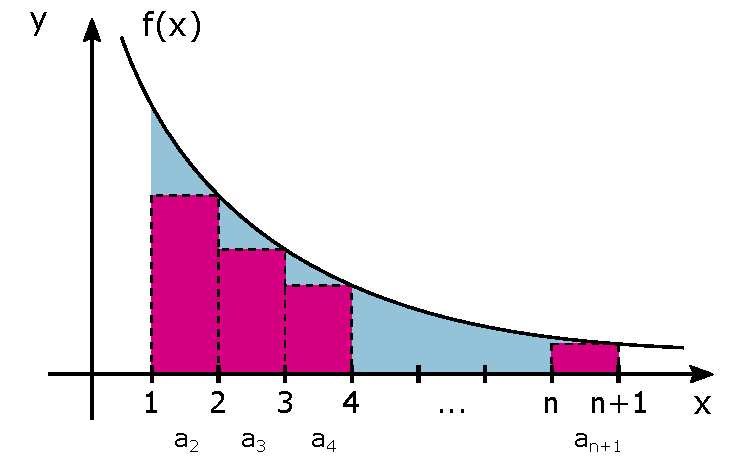
\includegraphics[scale=0.5]{thRow-Int.pdf}
\end{center}
Если интеграл $\int_1^{+\infty}f(x)dx$ сходится, то он представляет площадь под графиком $f(x)$ при $x\ge 1$. 
Сумма ряда $\displaystyle \sum_{k=2}^{+\infty}a_k$ можно интерпретировать, как площадь прямоугольников, полностью лежащих под графиком $f$. 

Следовательно, из ограниченности площади под графиком $f$ следует и ограниченность суммарной площади прямоугольников.
\end{frame}

\begin{frame}{Числовые ряды. Ряд Дирихле}
\begin{block}{Ряд Дирихле}
Ряд $\displaystyle \sum_{n=1}^{+\infty} \frac{1}{n^\alpha}$ сходится при $\alpha>1$ и расходится при $\alpha\le 1$.
\end{block}
\begin{block}{Доказательство}
При $\alpha\le 0$ ряд, очевидно, расходится. Пусть $\alpha>0$. Поскольку $f(x) = \frac{1}{x^\alpha}$ положительна, непрерывна и монотонно убывает, то применим интегральный признак сходимости. Таким образом, интеграл и ряд:
$$ \sum_{n=1}^{+\infty} \frac{1}{n^\alpha},\qquad \int_1^{+\infty}\frac{dx}{x^\alpha}$$
сходятся или расходятся одновременно. Мы знаем, что этот интеграл сходится при $\alpha>1$ и расходится при $0<\alpha \le 1$.
\end{block}
\begin{block}{Замечание}
Величину суммы ряда $\displaystyle  \zeta(\alpha) =\sum_{n=1}^{+\infty} \frac{1}{n^\alpha}$ называют функцией Римана. Она имеет ключевое значение в теории чисел.
\end{block}
\end{frame}

\begin{frame}{Числовые ряды}
\begin{block}{Пример}
Рассмотри ряд $\displaystyle \sum_{n=1}^{+\infty} \frac{\ln(n)}{\sqrt{n^3+5}}$. Заметим, что
$$\frac{\ln(n)}{\sqrt{n^3+5}} \sim \frac{\ln(n)}{n^{3/2}} =\frac{O(n^{1/4})}{n^{3/2}} = O \left( \frac{1}{n^{5/4}} \right).$$
Поскольку ряд $\displaystyle \sum_{n=1}^{+\infty} \frac{1}{n^{5/4}}$ сходится (ряд Дирихле), то сходится и исходный ряд (теорема об асимптотическом сравнении рядов).
\end{block}
\begin{block}{Упражнения}
Исследуйте сходимость рядов
$$\sum_{n=1}^{+\infty} \frac{1}{n \ln(n)},\qquad 
\sum_{n=1}^{+\infty} \frac{1}{n \ln^2(n)}.$$
Попробуйте применить к ним признаки Даламбера, Коши и интегральный признак сходимости.
\end{block}
\end{frame}

\begin{frame}{Числовые ряды. Знакопеременные ряды}
\begin{block}{Определение}
Числовой ряд называют {\bf знакопеременным}, если среди членов ряда имеется бесконечно много как положительных так и отрицательных членов. 
\end{block}
Действительно, иначе отбросив фиксированное число членов ряда мы бы получили знакопостоянный ряд.
\begin{block}{Определение}
Если сходится ряд $\displaystyle \sum_{n=1}^{+\infty}|a_n|$, то говорят, что ряд $\displaystyle \sum_{n=1}^{+\infty}a_n$ {\bf абсолютно сходится}. Если ряд сходится, но не является абсолютно сходящимся, то говорят, что ряд {\bf сходится условно}.
\end{block}
\begin{block}{Теорема}
Из абсолютной сходимости ряда следует сходимость ряда:
$$\sum_{n=1}^{+\infty}|a_n|<+\infty \quad \Rightarrow \quad \sum_{n=1}^{+\infty}a_n \ \text{--- сходится.}
$$
\end{block}
\end{frame}

\begin{frame}{Числовые ряды. Знакопеременные ряды}
\begin{block}{Определение}
Числовой ряд $\displaystyle \sum_{n=1}^{+\infty}(-1)^n a_n$, где $a_n\ge 0$, называют {\bf рядом Лейбница}. 
\end{block}
\begin{block}{Теорема. Признак Лейбница}
Пусть $a_n\ge 0$ монотонно стремятся к нулю:
$$a_n\to 0\quad (n\to+\infty),\qquad  a_{n+1}\le a_n \quad \forall n\in\mathbb{N}.$$
Тогда ряд Лейбница $\displaystyle \sum_{n=1}^{+\infty}(-1)^n a_n$ сходится.

Если ряд Лейбница сходится, то остаток ряда не превосходит первого отброшенного слагаемого:
$$\left| \sum_{n=N}^{+\infty}(-1)^n a_n \right| \le a_N \qquad \forall N\in\mathbb{N}.$$
\end{block}
\end{frame}

\begin{frame}{Числовые ряды. Знакопеременные ряды}
\begin{block}{Доказательство признака Лейбница}
Рассмотрим последовательность частичных сумм с нечетным числом слагаемых:
$$S_{2n+1} = -a_1+a_2-a_3+\cdots+a_{2n}-a_{2n+1} = S_{2n-1}+a_{2n}-a_{2n+1}\ge S_{2n-1}.$$
Таким образом, последовательность $S_{2n+1}$ монотонно возрастает, но
$$S_{2n+1} =-(a_1-a_2)-\cdots - (a_{2n-1}-a_{2n})-a_{2n+1} \le 0.$$
По теореме Вейерштрасса о монотонной ограниченной последовательности получаем, что
$$\exists\ \lim_{n\to+\infty}S_{2n+1} = S.$$
Следовательно,
$$\lim_{n\to+\infty}S_{2n} =\lim_{n\to+\infty}( S_{2n-1}+a_{2n}) = S+0 = S\quad \Rightarrow \quad S_{n}\to S.
$$
Мы доказали сходимость ряда. Докажем оценку для остаточного члена.
Последовательность $S_{2n}$ является монотонно убывающей. Следовательно,
$$S_{2n+1}\le S \le S_{2n+2}\le S_{2n} \quad \Rightarrow\quad
\left| \sum_{n=N}^{+\infty}(-1)^n a_n \right| = \left| S-S_{N-1} \right| \le \left| S_{N}-S_{N-1} \right|=a_N.$$
\end{block}
\end{frame}

\begin{frame}{Числовые ряды. Знакопеременные ряды}
\begin{block}{Пример}
Рассмотрим знакочередующийся ряд $\displaystyle \sum_{n=1}^{+\infty}\frac{(-1)^{n+1}}{n}$. Этот ряд не является абсолютно сходящимся, так как расходится ряд $\displaystyle \sum_{n=1}^{+\infty}\frac{1}{n}$. 
\vskip1em
Исследуем ряд на условную сходимость.
Последовательность $1/n$, очевидно, монотонно стремится к нулю. Применяя признак Лейбница, получаем, что ряд $\displaystyle \sum_{n=1}^{+\infty}\frac{(-1)^{n+1}}{n}$ сходится условно.
\end{block}
\end{frame}

\begin{frame}{Числовые ряды. Перестановка членов ряда}
\begin{block}{Определение}
\vskip-0.7em
Будем говорить, что ряд $\displaystyle \sum_{n=1}^{+\infty}b_n$ получен из ряда $\displaystyle \sum_{n=1}^{+\infty}a_n$, перестановкой слагаемых, если $b_n = a_{s(n)}$, где $s(n)$ --- биекция из $\mathbb{N}$ в $\mathbb{N}$.
\end{block}
\vskip-0.5em
\begin{block}{Теоремы о перестановке слагаемых}
Если ряд сходится абсолютно, то к той же сумме абсолютно сходится и ряд с переставленными слагаемыми.
\pause
\vskip0.7em
Если ряд является лишь условно сходящимся, то для любого числа $S$ существует такая перестановка слагаемых, что ряд с переставленными слагаемыми будет сходится к сумме $S$.
\pause
\vskip0.7em
Для заданного знакопеременного ряда рассмотрим суммы его положительных и отрицательных слагаемых:
$$A_{+} = \sum_{n:\ a_n>0} a_n,\qquad A_{-} = \sum_{n:\ a_n<0} |a_n|.$$
\vskip-1em
Ряд $\displaystyle \sum_{n=1}^{+\infty}a_n$ сходится абсолютно тогда и только тогда, когда сходятся положительные ряды~$A_{+}$ и $A_{-}$. В этом случае справедливо равенство для сумм: $A = A_{+} - A_{-}$.
\end{block}
\end{frame}

\begin{frame}{Функциональные последовательности. Определение}
\begin{block}{Определения}
Последовательность функций 
$$f_1(x),\ f_2(x),\ldots,$$
 где все функции $f_n(x)$ определены на общем множестве $x\in X\subset\mathbb{R}$, называют {\bf функциональной последовательностью}.
\vskip1em
Можно считать, что $\{ f_n(x) \}$ --- это семейство числовых последовательностей, зависящее от $x\in X$ как от параметра.
\vskip1em
Говорят, что функциональная последовательность $\{ f_n(x) \}$ {\bf сходится в точке} $x=x_0$, если сходится соответствующая числовая последовательность $\{ f_n(x_0) \}$.
\vskip1em
Пусть последовательность $\{ f_n(x) \}$ сходится для всех $x\in Y\subset X$. Тогда, очевидно, предел функциональной последовательности
$$f(x) = \lim_{n\to+\infty} f_n(x)$$
зависит от $x$. В этом случае говорят, что последовательность функций $\{ f_n \}$ {\bf поточечно сходится} к функции $f$ при $x\in Y$, функцию $f$ называют {\bf предельной функцией}.
\end{block}
\end{frame}

\begin{frame}{Функциональные последовательности. Пример}
\begin{block}{Пример}
Рассмотрим последовательность функций $\{ x^n \}$. Тогда
$$\lim_{n\to+\infty} x^n = \left\{ 
\begin{array}{ll}
0,& \text{ при $-1<x<1$;}\\
1,& \text{ при $x=1$;}\\
\nexists & \text{ при $x\not\in(-1,1]$}.
\end{array}\right.
$$
Следовательно, функциональная последовательность сходится на множестве $(-1,1]$.
\end{block}

\begin{block}{Замечание}
Из рассмотренного примера видно, что функциональная последовательность непрерывных функций не обязательно сходится к непрерывной функции.
\vskip1em
Так последовательность непрерывных функций $x^n$ сходятся на множестве $x\in(-1,1]$. Но предельная функция не является непрерывной в точке $x=1$.
\end{block}

\begin{block}{Упражнение}
Для последовательности $(1-x^2)^n$ определите множество сходимости и предельную функцию.
\end{block}
\end{frame}

\begin{frame}{Равномерная сходимость}
\begin{block}{Определение. Равномерная сходимость}
Говорят, что функциональная последовательность $\{ f_n(x) \}$ {\bf сходится равномерно} к функции~$f(x)$ при $x\in X$, если
$$\forall \varepsilon>0\ \exists N=N(\varepsilon):\quad  \forall n\ge N,\ \forall x\in X \quad \Rightarrow \quad | f(x) - f_n(x)|<\varepsilon.$$
\end{block}
Если записать определение поточечной сходимости на $X$, то получим
$$ \forall x\in X,\ \forall \varepsilon>0\ \exists N=N(\varepsilon,x):\quad  \forall n\ge N \quad \Rightarrow \quad | f(x) - f_n(x)|<\varepsilon.$$
Таким образом, равномерная сходимость является более сильным условием, так как требуется не только существование номера $N$, но и его независимость от $x$.
\begin{block}{Утверждение}
Последовательность $f_n(x)$ равномерно сходится  к $f(x)$ при $x\in X$ тогда и только тогда, когда
$$\sup_{x\in X}|f(x) - f_n(x)|\to 0\qquad (n\to+\infty).$$
\end{block}
\vskip-1.2em
\begin{block}{Доказательство}
$$\sup_{x\in X}|f(x) - f_n(x)|\le \varepsilon \quad \iff \quad \forall x\in X\quad |f(x) - f_n(x)|\le \varepsilon.$$
\end{block}
\end{frame}

\begin{frame}{Равномерная сходимость}
\begin{block}{Утверждение}
Из равномерной сходимости следует поточечная сходимость. Обратное, вообще говоря, не верно.
\end{block}
\begin{block}{Доказательство}
То, что из равномерной сходимости следует поточечная сходимость --- очевидно. Покажем на примере, что обратное не верно.
\end{block}
\pause
\begin{block}{Пример}
 Рассмотрим функциональною последовательность $x^n$ при $x\in(0,1)$, которая сходится поточечно к нулю. Пусть $x_n = 1-1/n$. Тогда $x_n\in(0,1)$ и $f_n(x_n) \to 1/e$ при $n\to+\infty$, следовательно, равномерной сходимости нет.
\vskip1em
Действительно, из равномерной сходимости следует, что $f_n(x)$ должна стремится к нулю при $n\to+\infty$ вне зависимости от выбора $x$, но $f_n(x_n) \to 1/e\ne0$.
\end{block}
\end{frame}

\begin{frame}{Функциональные ряды}
Аналогично с функциональными последовательностями рассматривают и функциональные ряды.
\begin{block}{Определение. Сходимость функционального ряда}
\vskip-1em
Пусть задана функциональная последовательность $\{ f_n(x)\}$. Тогда символ $\displaystyle \sum_{n=1}^{+\infty}f_n(x)$ называют {\bf функциональным рядом}.
Если для любого $x\in X$ сходится последовательность частичных сумм ряда
\vskip-0.6em
$$S_n(x) = \sum_{k=1}^{n}f_k(x)\to S(x),\qquad (n\to+\infty),$$
\vskip-0.4em
то говорят, что ряд {\bf сходится поточечно} при $x\in X$ и имеет сумму $S(x)$. Пишут:
\vskip-0.5em
$$\sum_{n=1}^{+\infty}f_n(x) = S(x).$$
\end{block}
\vskip-1.2em
\pause
\begin{block}{Определение. Равномерная сходимость}
\vskip-0.5em
Функциональный ряд $\displaystyle \sum_{n=1}^{+\infty}f_n(x)$ {\bf сходится равномерно} по $x\in X$ к сумме $S(x)$, если равномерно к $S(x)$ сходится последовательность частичных сумм ряда:
\vskip-0.5em
$$\forall \varepsilon>0\ \exists N=N(\varepsilon):\quad  \forall n\ge N,\ \forall x\in X \quad \Rightarrow \quad \left| \sum_{k=1}^n f_k(x) -S(x)\right|<\varepsilon.$$
\end{block}
\end{frame}

\begin{frame}{Свойства равномерно сходящихся последовательностей и рядов}
\begin{block}{Теорема (Непрерывность)}
Пусть последовательность непрерывных функций $\{ f_n(x) \}$ сходится равномерно к $f(x)$ на~$[a,b]$. Тогда функция $f(x)$ непрерывна на $[a,b]$.
\end{block}
\vskip-1em
\begin{block}{Теорема (Интегрирование)}
Пусть функциональная последовательность $\{ f_n(x) \}$ сходится равномерно к $f(x)$ при $x\in[a,b]$. Тогда, если функции $f_n(x)$ интегрируемы на отрезке $[a,b]$, то функция $f(x)$ также интегрируема на $[a,b]$ и
$$ \exists\ \lim_{n\to+\infty} \int_a^b f_n(x)dx = \int_a^b f(x)dx.$$
\end{block}
\vskip-1em
\begin{block}{Теорема (Дифференцирование)}
Пусть функциональная последовательность непрерывно дифференцируемых функций $\{ f_n(x) \}$ сходится к $f(x)$ при $x\in[a,b]$ и последовательность производных  $\{ f'_n(x) \}$ сходится равномерно на $[a,b]$. Тогда функция $f(x)$ непрерывно дифференцируема на $[a,b]$ и
$$ \lim_{n\to+\infty}f'_n(x)= f'(x)$$
\end{block}
Аналогичные утверждения справедливы и для функциональных рядов.
\end{frame}

\begin{frame}{Признак равномерной сходимости ряда}
\begin{block}{Теорема Вейерштрасса}
Пусть задан функциональный ряд $\ \displaystyle \sum_{n=1}^{+\infty}f_n(x)$ при $x\in X$ и сходящийся числовой ряд $\ \displaystyle \sum_{n=1}^{+\infty}a_n$. Если справедливы неравенства:
$$|f_n(x)|\le a_n,\quad \forall n\in\mathbb{N},\ \forall x\in X,$$
то функциональный ряд сходится равномерно в $X$.
\end{block}
В этом случае числовой ряд $\ \displaystyle \sum_{n=1}^{+\infty}a_n$ называют {\bf мажорирующим} для ряда $\ \displaystyle \sum_{n=1}^{+\infty}f_n(x)$.
\end{frame}

\begin{frame}{Степенные ряды}
\begin{block}{Определение степенного ряда}
Функциональный ряд $\ \displaystyle \sum_{n=0}^{+\infty}a_n (x-x_0)^n\ $ называют {\bf степенным рядом} с центром в точке $x_0$. Последовательность $a_n$ называют {\bf последовательностью коэффициентов} степенного ряда.
\end{block}
\vskip1em
Простой заменой переменных $\tilde x = x-x_0$ можно перейти к рассмотрению степенного ряда~$\ \displaystyle \sum_{n=0}^{+\infty}a_n \tilde x^n$ с центром в точке $\tilde x=0$.
\vskip1em
\begin{block}{Определение ряда Тейлора}
{\bf Рядом Тейлора} функции $f(x)$, дифференцируемой любое число раз в окрестности точки~$x_0$, называют степенной ряд
$$ \sum_{n=0}^{+\infty}\frac{f^{(n)}(x_0)}{n!}(x-x_0)^n = f(x_0) + \frac{f'(x_0)}{1!}(x-x_0)+ \frac{f''(x_0)}{2!}(x-x_0)^2+\cdots$$
\end{block}
\end{frame}

\begin{frame}{Степенные ряды}

\begin{block}{Пример}
Бесконечная геометрическая прогрессия сходится при $|x|<1$:
\vskip-0.3em
$$\sum_{k=0}^{+\infty} x^k = \frac{1}{1-x}.$$
\vskip-0.2em
Сходимость не является равномерной на $(-1,1)$. Действительно
\vskip-0.2em
$$\frac{1}{1-x} - \sum_{n=1}^n x^n = \frac{1}{1-x} -\frac{1-x^{n+1}}{1-x} = \frac{x^{n+1}}{1-x}.$$
\vskip-0.1em
Равномерная сходимость на $(-1,1)$ эквивалентна (по утверждению):
$$\sup_{x\in(-1,1)}\ \left| \frac{x^{n+1}}{1-x} \right|\to 0,\qquad (n\to+\infty)$$
но $\sup$ равен $+\infty$ для каждого $n$.
\vskip0.6em
С другой стороны, равномерная сходимость имеет место для любого отрезка~$[-r,r]\subset(-1,1)$, поскольку:
$$ \sup_{x\in[-r,r]}\ \left| \frac{x^{n+1}}{1-x} \right|=
\frac{|r|^n}{1-r}\to 0, \qquad (n\to+\infty).$$
\end{block}
\end{frame}

\begin{frame}{Степенные ряды}
\begin{block}{Теорема о множестве сходимости степенного ряда}
Если степенной ряд $\ \displaystyle \sum_{n=0}^{+\infty}a_n x^n$ сходится для $x_0\ne 0$, то он абсолютно сходится для любого~$|x_1|<|x_0|$. Ряд равномерно сходится на отрезке $[-r,r]$, где $r=|x_1|$.
\end{block}
\begin{block}{Доказательство}
По условию ряд $\ \displaystyle \sum_{n=0}^{+\infty}a_n x_0^n$ сходится. Следовательно,
$$a_n x_0^n\to 0,\quad n\to+\infty \quad \Rightarrow \quad \exists M:\ |a_n x_0^n|<M,\quad \forall n\in\mathbb{N}.$$
Пусть $|x_1|<|x_0|$. Тогда
$$|a_n x_1^n|= |a_n x_0^n| \left| \frac{x_1}{x_0} \right|^n \le M\ q^n,$$
где $q = \left| \frac{x_1}{x_0} \right|<1$. По признаку сравнения ряд  $\ \displaystyle \sum_{n=0}^{+\infty}|a_n x_1^n|$ сходится. Равномерная сходимость на $[-r,r]$ следует из признака Вейерштрасса.
\end{block}
\end{frame}

\begin{frame}{Радиус сходимости степенного ряда}
\begin{block}{Определение}
\vskip-0.5em
Рассмотрим множество $X$ сходимости степенного ряда  $\ \displaystyle \sum_{n=0}^{+\infty}a_n x^n$. 

{\bf Радиусом сходимости} степенного ряда называют величину
$$R = \sup_{x\in X}|x|.$$
Множество $X$ всегда не пусто, поскольку $0\in X$.
\vskip1em
Если $R=0$, то есть степенной ряд сходится только для $x=0$, то его называют {\bf всюду расходящимся}.
\vskip1em
Если множество $X$ не является ограниченным и, следовательно, $R=+\infty$, то степенной ряд (по теореме) сходится для любых $x\in\mathbb{R}$. Такой ряд называют {\bf всюду сходящимся}.
\end{block}
\vskip-0.8em
\begin{block}{Следствия}
Из доказанной теоремы следует, что интервал $(-R, R)$ всегда лежит в множестве сходимости степенного ряда $X$. На интервале $(-R, R)$ степенной ряд сходится абсолютно и ряд расходится вне этого интервала. Ряд сходится равномерно на любом отрезке $[-r,r]$, который полностью лежит в интервале сходимости $(-R,R)$.
\end{block}
\end{frame}

\end{document}